% Issue #76; owner: MilindDevX. Input from reports/phase2/main.tex.
% Numbers: results/metrics/fd001_validation_*.{csv,json} (notebooks/phase2/13_validation.ipynb, #72),
% fd001_final_test*.{json,csv} (#71) and fd00{2,4}_test_*.json, fd002_fd004_multi_regime_*.csv
% (notebooks/phase2/12_multi_regime.ipynb, #70). Tables: tables/validation_*.tex and
% tables/multi_regime_test.tex, generated by scripts/prepare_validation_tables.py.

\section{Technical Validation}
\label{sec:validation}

The earlier sections chose every model and setting by cross-validation on the
training engines. This section reports how those choices hold up on the
official test set, which was scored once after the model freeze, and asks
which differences between models are larger than the noise in the
evaluation.

\subsection{Method}
\paragraph{One test run}
At the freeze commit, every model was trained on all 100 training engines
with its final settings. Each network trained for the median best epoch of
the cross-validation that tuned it. The networks were trained at five seeds
(42--46), both with the cap of 125 and uncapped. The ML baselines were trained
once, at seed 42, with the settings chosen in cross-validation. Each test
engine is scored once, at its last recorded cycle, against its true, uncapped
RUL. A checked guard stops the notebook if any model code or configuration
differs from the freeze commit, and later runs only reload the saved
predictions.

\paragraph{Uncertainty}
Two sources of noise are measured separately. The standard deviation over
seeds shows how much a network depends on its random initialization. The
bootstrap 95\% confidence interval resamples the 100 test engines 10{,}000
times~\cite{Efron1993introduction}, and shows how much a score depends on
which engines happen to be in the test set.

\paragraph{Paired comparisons}
Three comparisons were fixed before the test was read, all from
cross-validation results. The best sequence model, the Transformer, is
compared with the best ML model, XGBoost on engineered features. Each hybrid
is compared with the single branch that was best in the hybrid study: the
LSTM for Hybrid~A, and XGBoost on the engineered features for Hybrid~B. Each
comparison reports the paired bootstrap interval on the RMSE difference and a
Wilcoxon signed-rank test on the per-engine absolute
errors~\cite{Wilcoxon1945individual}. The three tests form one family under
Holm's correction~\cite{Holm1979simple}.

\paragraph{The value test}
The team fixed this test before any hybrid was trained. A hybrid adds value
over its best single branch only if at least one of the following holds:
(1)~the paired bootstrap interval on the RMSE difference lies below zero;
(2)~the Holm-corrected Wilcoxon test gives $p<0.05$ with the hybrid's median
error lower; or (3)~its RMSE varies less across seeds, with a mean that is no
worse. Otherwise the result is null.

\subsection{Results on FD001}

\begin{table*}[t]
\centering
\caption{Official FD001 test, 100 engines scored at their last cycle.
RMSE: mean $\pm$ s.d.\ over seeds (one run for the ML baselines). 95\% CI:
bootstrap over engines for the seed-averaged RMSE. All models are trained
with the cap of 125 except the last column.}
\label{tab:validation_models}
\footnotesize
% Generated by scripts/prepare_validation_tables.py from the #71 test predictions
% (results/metrics/fd001_final_test_predictions.csv, fd001_ml_capped_test_predictions.csv),
% as in notebooks/phase2/13_validation.ipynb (#72). Do not edit by hand.
\begin{tabular}{@{}lccccc@{}}
\hline
Model & Seeds & RMSE & 95\% CI & MAE & RMSE, uncapped \\
\hline
Hybrid B, two-stage & 5 & 15.18 $\pm$ 0.55 & [12.79, 17.47] & 11.28 & 25.86 $\pm$ 1.07 \\
Hybrid A, gated & 5 & 15.40 $\pm$ 0.46 & [13.15, 17.73] & 11.89 & 27.52 $\pm$ 1.10 \\
Transformer & 5 & 15.60 $\pm$ 0.35 & [13.38, 17.72] & 11.91 & 30.30 $\pm$ 4.15 \\
XGBoost, engineered & 1 & 15.71 & [13.24, 18.05] & 11.59 & 28.56 \\
Temporal CNN & 5 & 15.83 $\pm$ 0.55 & [13.73, 17.88] & 12.10 & 29.85 $\pm$ 3.52 \\
LSTM & 5 & 15.95 $\pm$ 0.33 & [13.49, 18.36] & 11.96 & 28.97 $\pm$ 4.98 \\
Random Forest, engineered & 1 & 16.21 & [13.64, 18.64] & 11.95 & 27.55 \\
XGBoost, raw & 1 & 17.58 & [14.70, 20.20] & 12.78 & 24.83 \\
Elastic Net, engineered & 1 & 17.80 & [15.83, 19.62] & 14.83 & 28.39 \\
Random Forest, raw & 1 & 18.42 & [15.57, 21.07] & 13.75 & 26.15 \\
Elastic Net, raw & 1 & 22.44 & [19.35, 25.44] & 17.76 & 29.64 \\
\hline
\end{tabular}

\end{table*}

\begin{table*}[t]
\centering
\caption{Paired comparisons on the official FD001 test, cap 125. $\Delta$:
RMSE of A minus B, paired bootstrap 95\% CI. $p_\mathrm{Holm}$: Wilcoxon
signed-rank on per-engine absolute error, Holm-corrected over the three
comparisons. (1)--(3): the value-test criteria, for the hybrids only.
Criterion~(3) cannot be judged for Hybrid~B, whose branch ran with one
seed.}
\label{tab:validation_paired}
\footnotesize
% Generated by scripts/prepare_validation_tables.py from
% results/metrics/fd001_validation_value_test.json (#72). Do not edit by hand.
\begin{tabular}{@{}llcccccl@{}}
\hline
A & B & $\Delta$ [95\% CI] & $p_\mathrm{Holm}$ & (1) & (2) & (3) & Verdict \\
\hline
Hybrid A & LSTM & $-$0.54 [$-$3.35, $+$2.24] & 1.00 & no & no & no & null \\
Hybrid B & XGBoost, engineered & $-$0.53 [$-$1.45, $+$0.38] & 1.00 & no & no & n/a & null \\
Transformer & XGBoost, engineered & $-$0.11 [$-$2.42, $+$2.26] & 1.00 & -- & -- & -- & tie \\
\hline
\end{tabular}

\end{table*}

\begin{figure*}[t]
\centering
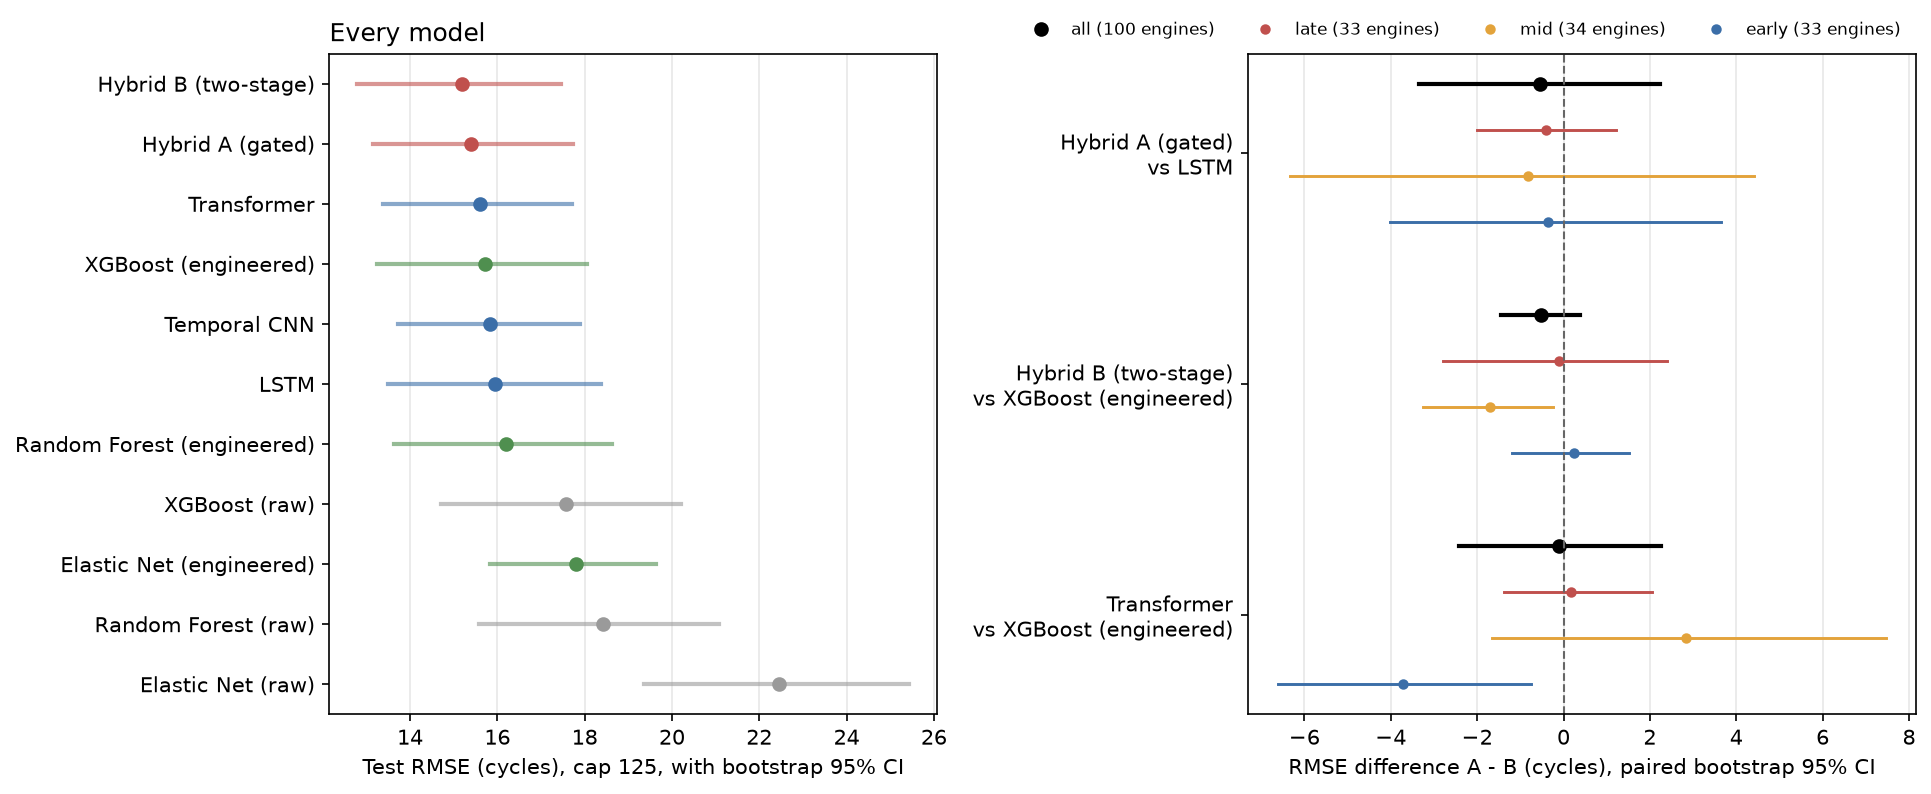
\includegraphics[width=\textwidth]{../../results/figures/fd001_validation.png}
\caption{Left: test RMSE of every model trained with the cap, with its
bootstrap 95\% CI over engines. Right: the three paired differences, A minus
B, over all engines and within each life stage. Left of zero favours A. The
stage intervals are not corrected for multiple tests.}
\label{fig:validation}
\end{figure*}

Table~\ref{tab:validation_models} and Fig.~\ref{fig:validation} show that
the test set cannot separate the final models. The seven best models score
between 15.18 and 16.21 cycles, a range of about one cycle, while each model's
confidence interval is 4 to 5 cycles wide. With 100 test engines, models this
close cannot be ranked.

Table~\ref{tab:validation_paired} gives the three fixed comparisons. All three
end in a tie or a null result, and every corrected $p$ is 1.
\begin{itemize}
\item \emph{Sequence against ML.} The Transformer is 0.11 cycles better than
XGBoost on engineered features, with an interval of $-2.42$ to $+2.26$. On
FD001, learning from raw sensor windows matches the engineered features with
boosted trees, but does not beat them.
\item \emph{Hybrid~A.} It is 0.54 cycles better than the LSTM, with an
interval of $-3.35$ to $+2.24$, and no criterion holds. In cross-validation
it passed criterion~(3), with a lower seed spread than the LSTM. On the test
it varies more (0.46 against 0.33), so that pass does not carry over.
\item \emph{Hybrid~B.} It is 0.53 cycles better than XGBoost, with an interval
of $-1.45$ to $+0.38$. This repeats the null result from cross-validation:
the LSTM embeddings add nothing measurable to the engineered features.
\end{itemize}

Two stage-wise differences exclude zero but are not corrected for the nine
stage comparisons, so we report them only as leads. In mid life, Hybrid~B is
1.69 cycles better than XGBoost (interval $-3.25$ to $-0.25$). Early in life,
the Transformer is 3.72 cycles better than XGBoost ($-6.61$ to $-0.75$).
Near failure, no comparison differs, and every network and tree model on
engineered features has an RMSE between 5.1 and 7.6 cycles. Two choices
matter more than the model family. On raw inputs, every ML model is 1.9 to
4.6 cycles worse. Training uncapped costs every model 7 to 15 cycles, and the
uncapped LSTM, temporal CNN and Transformer vary by 3.5 to 5.0 cycles across seeds.

\subsection{FD002 and FD004}
FD001 runs at one operating condition, so per-regime scaling cannot help
there. FD002 and FD004 run at six. Scaling each sensor within its regime
removes the jumps caused by the operating condition rather than by wear. On
these subsets, the sensor selection now keeps a sensor only if it varies
within at least one regime. That removes four sensors that change only with
the condition (21 to 17), while FD001 keeps its 15.

In cross-validation (seed 42, settings tuned on FD001), per-regime scaling
improved the LSTM on both subsets. The paired differences were $-1.30$ cycles
on FD002 (95\% CI $-1.83$ to $-0.75$) and $-3.20$ on FD004 ($-4.01$ to
$-2.40$), both with Holm-corrected $p<0.001$. It also improved Hybrid~A on
FD004 ($-3.17$), but made no clear difference on FD002 ($+0.43$, interval
$-0.72$ to $+1.67$). This agrees in direction with Gupta~\cite{Gupta2026auditing},
who found a larger effect on FD004 than on FD002 (mean test-set changes of
$-7.40$ and $-4.39$). Each model's better scaling was then scored once on the
official test, at seeds 42--44 (Table~\ref{tab:multi_regime_test}).

\begin{table*}[t]
\centering
\caption{Official FD002 and FD004 test (259 and 248 engines), seeds 42--44.
Scaling: the setting chosen by cross-validation. The last three columns split
the error at the training cap: RMSE on engines whose true RUL at the last
cycle is at most 125, RMSE on those above it, and the share above it.}
\label{tab:multi_regime_test}
\footnotesize
% Generated by scripts/prepare_validation_tables.py from
% results/metrics/fd00{2,4}_test_*.json and predictions (#70). Do not edit by hand.
\begin{tabular}{@{}lllccccc@{}}
\hline
Subset & Model & Scaling & RMSE & NASA & RMSE, $y\leq125$ & RMSE, $y>125$ & $y>125$ \\
\hline
FD002 & LSTM & per-regime & 26.58 $\pm$ 0.41 & 7{,}927 & 14.86 & 49.28 & 22\% \\
FD002 & Hybrid A & global & 27.01 $\pm$ 0.80 & 10{,}463 & 14.87 & 50.29 & 22\% \\
FD004 & LSTM & per-regime & 27.02 $\pm$ 0.61 & 4{,}993 & 15.62 & 45.19 & 27\% \\
FD004 & Hybrid A & per-regime & 26.88 $\pm$ 0.34 & 5{,}944 & 16.86 & 43.66 & 27\% \\
\hline
\end{tabular}

\end{table*}

On both subsets, the LSTM and Hybrid~A score within half a cycle of each
other (26.58 to 27.02), which is about their seed spread. Our best runs are
4 to 5 cycles behind Gupta's best configurations (22.73 on FD002 and 21.78 on
FD004). Most of our error comes from engines above the cap. On these
subsets, 22--27\% of the test engines have a true RUL above 125, up to 195. A
model trained with the cap rarely predicts much above 125, so it misses those
engines by 44 to 50 cycles RMSE and predicts too early on average. On the
engines at or below the cap, its RMSE is 14.9 to 16.9. Gupta's best
configurations use a cap of 150 and a window of 50, while ours keep the
FD001 settings. The cap is therefore the likely main cause of the gap, but a
cap of 150 was not run here, so this is not tested. Only the chosen scaling
was scored on the test, so the comparison between per-regime and global
scaling rests on cross-validation.

\subsection{What the Validation Supports}
On FD001, the sequence models, the hybrids and boosted trees on engineered
features are equally accurate within the precision this test set allows.
No hybrid passes the value test on the official test, so we report a null
result for both. The claims the evidence does support are about the
pipeline rather than the architecture. The training cap, the engineered
inputs and, on multi-regime data, per-regime scaling each change the error by
several cycles, more than any choice of model family.
